
We begin with an empirical investigation of \macroName{} in a multi-armed bandit, a
%n extremely
well-studied special case of the MDP where the state space $\Scal$ is a singleton and the horizon $H = 1$ is a single step. We will examine the performance of \macroName{} both when aiming to select a good action from offline historical data and for online learning where the goal is to maximize cumulative reward from scratch. Offline, it is critical to account for uncertainty due to noise as certain actions may not be sampled well enough. Online, it is critical to judiciously balance exploration and exploitation to minimize overall regret. For detailed descriptions of the experiment setups, see Appendix~\ref{app:experiment-details}.


\textbf{Pretraining distribution.} For the pretraining task distribution $\pretraint$, we sample $5$-armed bandits ($|\Acal| = 5$). The reward function for arm $a$ is a normal distribution $R(\cdot | s,a) = \Ncal(\mu_a, \sigma^2)$ where $\mu_a \sim \unif[0, 1]$ independently and $\sigma = 0.3$. To generate in-context datasets $\pretraind$, we randomly generate action frequencies by sampling probabilities from a Dirichlet distribution and mixing them with a point-mass distribution on one random arm (see details in Appendix~\ref{app:bandit-pretrain-data}). Then we sample the actions accordingly from  this distribution. This encourages diversity of the in-context datasets. The optimal policy $\pistar_{\tau}$ for bandit $\tau$ is $\argmax_{a} \mu_a$, which we can easily compute during pretraining. We pretrain the model $M_{\theta}$ to predict $a^\star$ from $D$ as described in Section~\ref{sec:in-context} for datasets up to size $n = 500$.

\textbf{Comparisons.}
We compare to several well-known algorithms for bandits\footnote{See Appendix~\ref{app:comparisons} for additional details such as hyperparameters.}. All of the algorithms are designed to reason in a particular way about uncertainty based on their observations.
\begin{itemize}[leftmargin=1em,noitemsep]
\item Empirical mean algorithm (Emp) selects the action with the highest empirical mean reward naively.
\item Upper Confidence Bound (UCB) selects the action with the highest  upper confidence bound. 
\item Lower Confidence Bound (LCB) selects the action with the highest lower confidence bound. 
\item Thompson Sampling (TS) selects the action with the highest sampled mean from a posterior distribution over reward models. The prior and likelihood functions are Gaussian.
\end{itemize}
Emp and TS~\citep{russo2018tutorial,thompson1933likelihood} can both be used for offline or online learning; UCB \citep{auer2002finite} is known to be provably optimal online by ensuring exploration through optimism under uncertainty; and LCB \citep{xiao2021optimality,jin2021pessimism} is  used to minimize suboptimality given an offline dataset by selecting actions pessimistically. It is the opposite of UCB. We evaluate algorithms with standard bandit metrics. Offline, we use the suboptimality $\mu_{a^\star} - \mu_{\hat a}$ where $\hat a$ is the chosen action. Online, we use  cumulative regret: $\sum_{k} \mu_{a^\star} - \mu_{\hat a_k}$ where $\hat a_k$ is the $k$th action chosen.

\begin{figure}
    \centering
    \begin{subfigure}{0.33\textwidth}
        \centering
        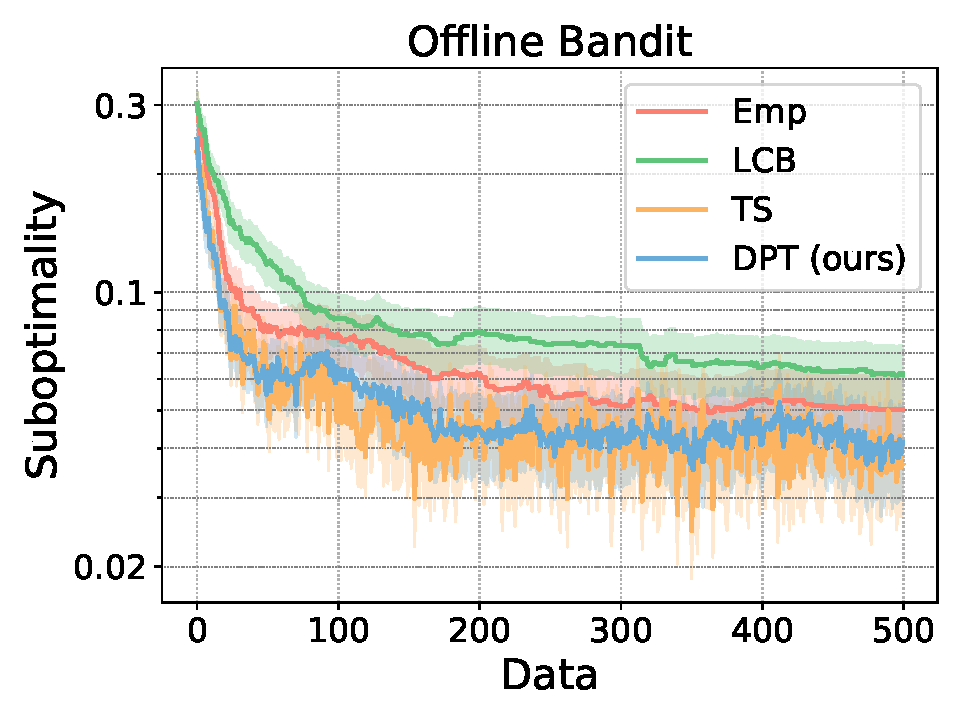
\includegraphics[width=\linewidth]{figures/bandit_offline_epoch300.pdf}
        \caption{}
        \label{fig:basic-offline}
    \end{subfigure}
    \begin{subfigure}{0.33\textwidth}
        \centering
        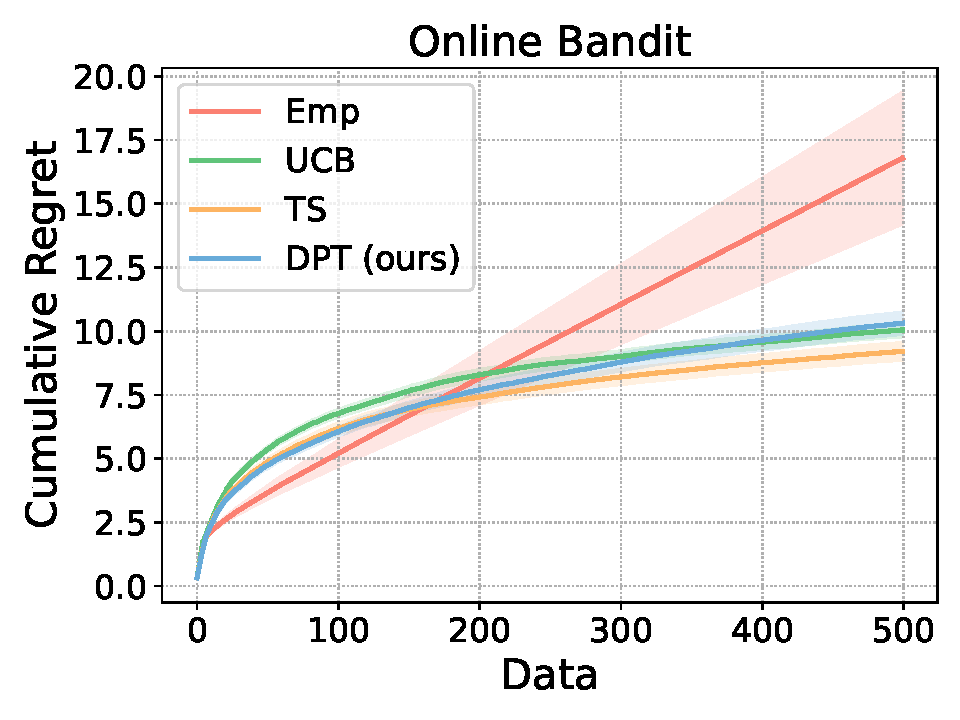
\includegraphics[width=\linewidth]{figures/bandit_online_epoch300.pdf}
        \caption{}
        \label{fig:basic-online}
    \end{subfigure}
\begin{subfigure}{0.32\textwidth}
  \centering
  % 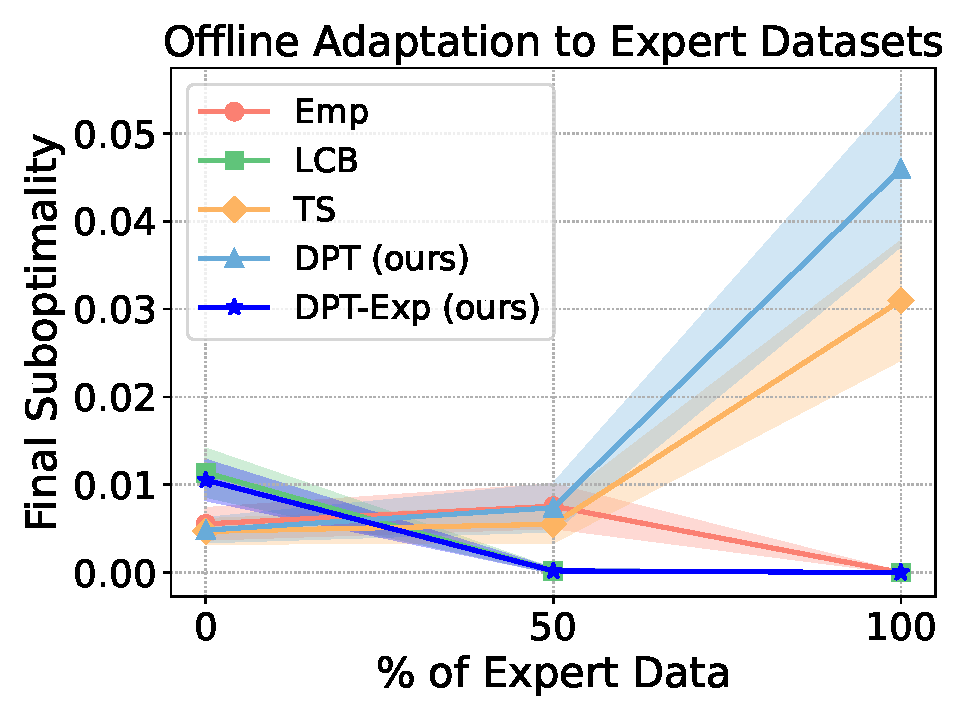
\includegraphics[width=\linewidth]{figures/bandit_offline_covs_epoch300_line.pdf}
    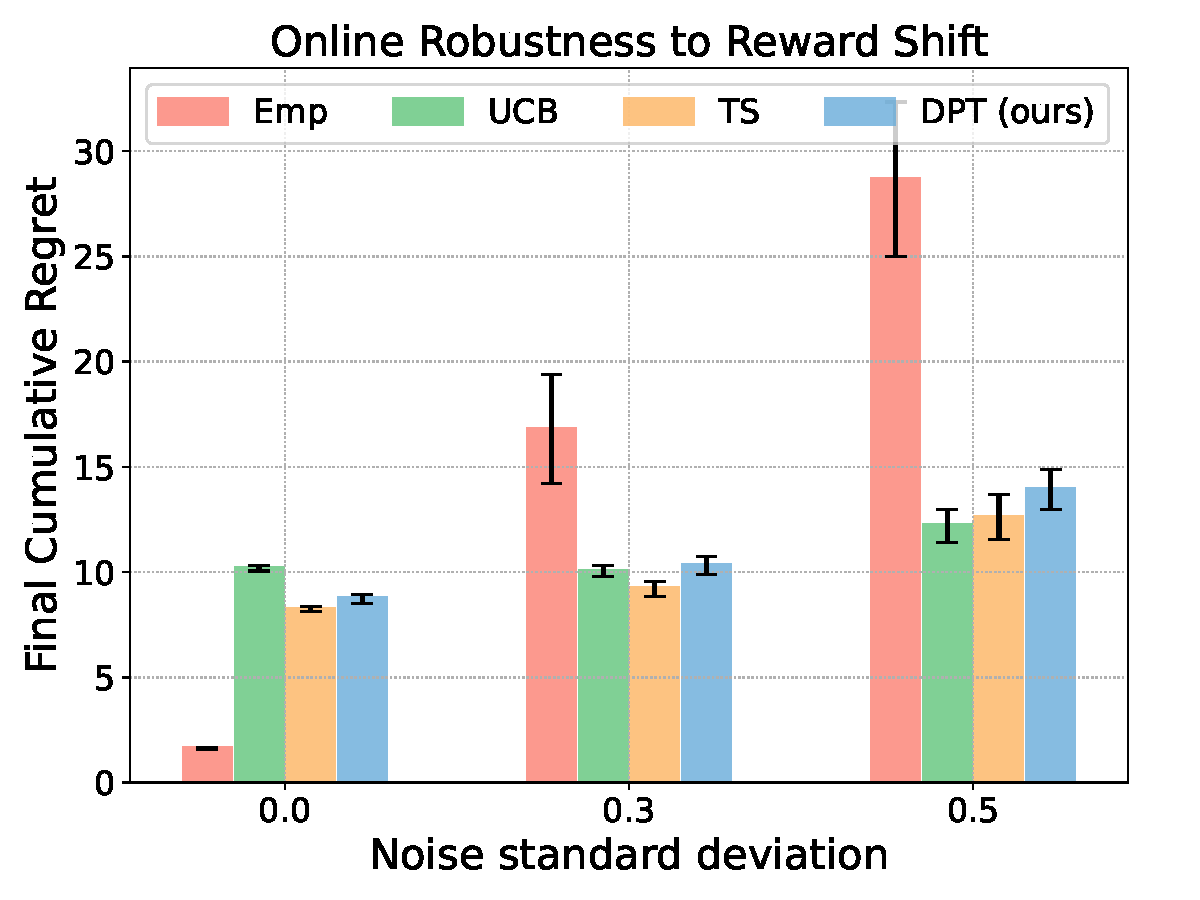
\includegraphics[width=\linewidth]{figures/bandit_online_vars_epoch300.pdf}
  \caption{}
  \label{fig:online-vars}
\end{subfigure}
\vspace{-0.1cm}
    \caption{\small (a) Offline performance on in-distribution bandits, given random in-context datasets. (b) Online cumulative regret on bandits. (c) Final (after 500 steps) cumulative regret on out-of-distribution bandits with different Gaussian noise standard deviations. The mean and standard error are computed over $200$ test tasks.}
    \vspace{-0.4cm}
\end{figure}
\textbf{DPT learns to reason through uncertainty.}
As shown in Figure~\ref{fig:basic-offline}, in the offline setting, DPT significantly exceeds the performance of Emp and LCB while matching the performance of TS, when the in-context datasets are sampled from the same distribution as during pretraining. The results suggest that the transformer is capable of reasoning through uncertainty caused by the noisy rewards in the dataset. 
Unlike Emp which can be fooled by noisy, undersampled actions, the transformer has learned to \emph{hedge} to a degree. However, it also suggests that this hedging is fundamentally different from what LCB does, at least on this specific distribution\footnote{Note our randomly generated environments are equally likely to have expert-biased datasets and adversarial datasets, so LCB is not expected to outperform here~\citep{xiao2021optimality}.}.

Interestingly, the same transformer produces an extremely effective online bandit algorithm when sampling actions instead of taking an argmax. As shown in Figure~\ref{fig:basic-online}, DPT matches the performance of classical optimal algorithms, UCB and TS, which are specifically designed for exploration. This is notable because \macroName{} was not explicitly trained to explore, but its emergent strategy is on par with some of the best.  In Figure~\ref{fig:online-vars}, we show this property is robust to noise in the rewards not seen during pretraining by varying the standard deviation. In Appendix~\ref{app:more-exps}, we show this generalization happens offline too and even with unseen Bernoulli rewards. 



\textbf{Leveraging structure from suboptimal data.} We now investigate whether \macroName{} can learn to leverage the inherent structure of a problem class, even without prior knowledge of this structure and even when learning from in-context datasets that do not explicitly utilize it. More precisely, we consider $\pretraint$ to be a distribution over \emph{linear} bandits, where the reward function is given by $\E\left[r \ | \ a, \tau \right] =  \dotp{\theta_\tau}{\phi(a)}$ and $\theta_\tau \in \RR^d$ is a task-specific parameter vector and $\phi: \Acal \to \RR^d$ is fixed feature vector that is the same for all tasks. 
Given the feature representation $\phi$, LinUCB~\citep{abbasi2011improved}, a UCB-style algorithm that leverages $\phi$, should achieve regret $\widetilde{\Ocal}(d\sqrt{ K})$ over $K$ steps, a substantial gain over UCB and TS when $d \ll |\Acal|$. %For the pretraining dataset $\pretraind$ to
Here, we pretrain a \macroName{} model with in-context datasets gathered by TS, which does not leverage the linear structure. Figures~\ref{fig:struct-offline} and~\ref{fig:struct-online} show that \macroName{} can exploit the unknown linear structure, essentially learning a surrogate for $\phi$, allowing to do more informed exploration online and decision-making offline. 
It is nearly on par with LinUCB (which is given $\phi$) and significantly outperforms the dataset source, TS, which does not know or use the structure. These results present evidence that (1) \macroName{} can automatically leverage structure, and (2) supervised learning-based approaches to RL \emph{can} learn novel explorations that transcend the quality of their pretraining data. 


\textbf{Adapting to expert-biased datasets.}
A common assumption in offline RL is that datasets tend to be a mixture between optimal data (e.g. expert demonstrations) and suboptimal data (e.g. random interactions)~\citep{rashidinejad2021bridging}. Hence, LCB is generally effective in practice and the pretraining and testing distributions should be biased towards this setting. Motivated by this, we 
pretrain a second \macroName{} model where $\pretraind$ is generated by mixing the in-context datasets with varying fractions of expert data, biasing $\pretraind$ towards datasets that contain more examples of the optimal action. We denote this model by \macroName{}-Exp. In Figure~\ref{fig:bandit-exp}, we plot the test-time performance of both pretrained models when evaluated on new offline datasets with varying percentages of expert data\footnote{That is, $0\%$ is fully random while $100\%$ has only optimal actions in the in-context dataset.}. Our results suggest that when the pretraining distribution is also biased towards expert-suboptimal data, \macroName{}-Exp behaves similarly to LCB, while \macroName{} continues to resemble TS. This is quite interesting as for other methods, such as TS, it is less clear how to automatically incorporate the right amount of expert bias to yield the same effect, but \macroName{} can leverage this from pretraining.






\begin{figure}
    \centering
    \begin{subfigure}{0.32\textwidth}
        \centering
        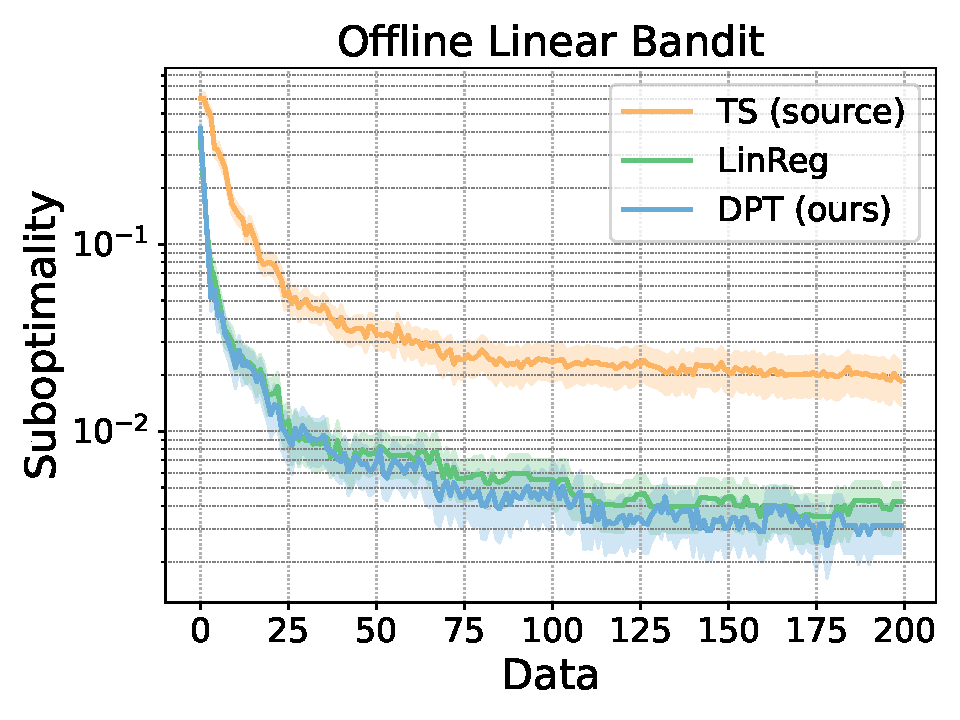
\includegraphics[width=\linewidth]{figures/bandit_offline_epoch200.pdf}
        \caption{}
        \label{fig:struct-offline}
    \end{subfigure}
    \begin{subfigure}{0.32\textwidth}
        \centering
        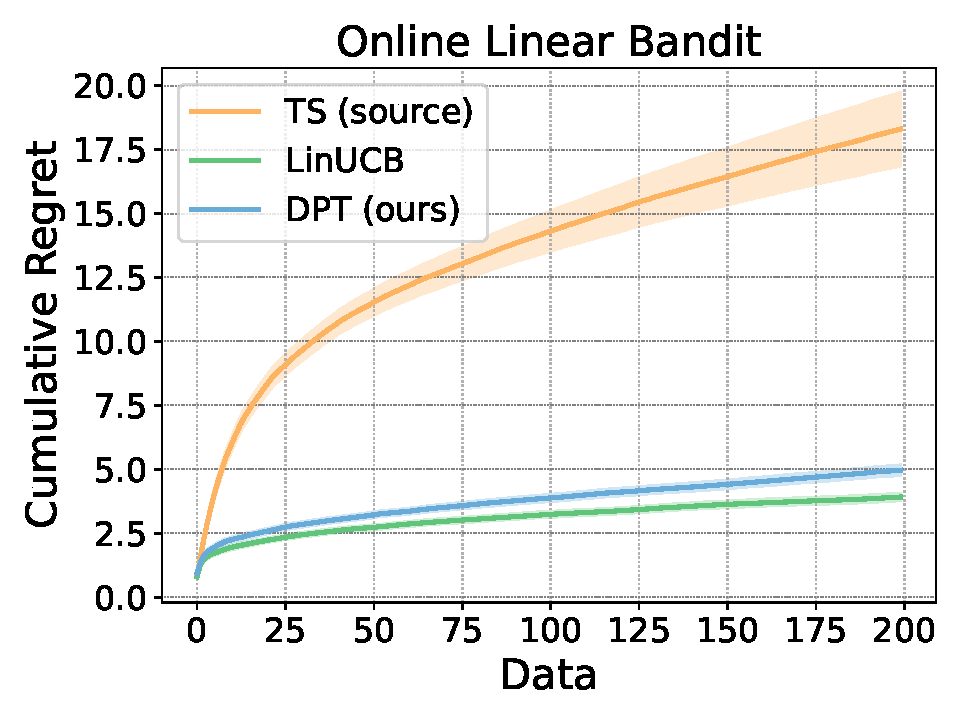
\includegraphics[width=\linewidth]{figures/bandit_online_epoch200.pdf}
        \caption{}
        \label{fig:struct-online}
    \end{subfigure}
    \begin{subfigure}{0.32\textwidth}
        \centering
        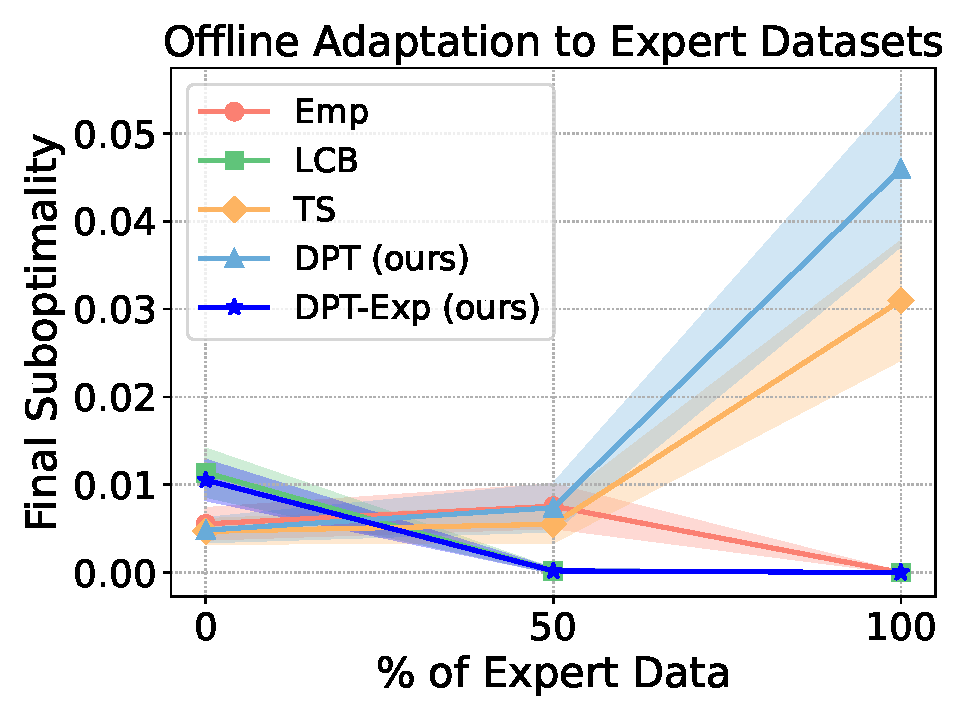
\includegraphics[width=\linewidth]{figures/bandit_offline_covs_epoch300_line.pdf}
        \caption{}
        \label{fig:bandit-exp}
    \end{subfigure}

    \vspace{-0.1cm}
    \caption{\small 
    (a) Offline performance of DPT trained on linear bandits from TS source data. LinReg does linear regression and outputs the greedy action. (b) Online cumulative regret of the same model. The mean and standard error are computed over $200$ test tasks. (c) Offline performance on expert-biased datasets. DPT pretrained on a different prior continues to match TS, but DPT-Exp trained from a more representative prior excels.}
    \vspace{-0.4cm}
\end{figure}

